\documentclass[11pt]{article}
\usepackage[utf8]{inputenc}
\usepackage{graphicx}
\usepackage{a4wide}
\usepackage[square, numbers]{natbib}
\usepackage{algpseudocode}
\usepackage{boxedminipage}
\usepackage{amsthm}
\usepackage{amsmath}
\usepackage{amsfonts}
\usepackage{amssymb}
\usepackage{tikz}
\usepackage{multirow}

\usepackage[
bookmarks=true,
colorlinks=true,
breaklinks=true,
urlcolor=red,
citecolor=blue,
linkcolor=blue,
unicode=true,
]
{hyperref}

%\renewcommand*\rmdefault{iwona}

\paperwidth=210 true mm
\paperheight=297 true mm
\pdfpagewidth=210 true mm
\pdfpageheight=297 true mm

\author{Daniel Meister and Ji\v{r}i Bittner}
\title{Time-Varying Appearance}

\begin{document}

\begin{center}
\textsc{\LARGE Time-Varying Appearance}\\[0.4cm]
\textsc{\Large Technical Report - February 2018}\\[0.4cm]
\textsc{\large Toyota Research Lab}\\[0.4cm]
\textsc{\normalsize Daniel Meister and Ji\v{r}i Bittner}\\[0.5cm]
\end{center}

\section{Introduction}

\section{Related Work}
Traditionally, various phenomena have been studied individually weathering effects and proposed models based on physically inspired simulations: metallic patinas \cite{Dorsey1996a}, flow of water \cite{Dorsey1996b}, stone weathering \cite{Dorsey1999,Xue2011}, lichen growth \cite{Desbenoit2004}, peeling and cracking \cite{Paquette2002}, dust accumulation \cite{Hsu1995}, scratches \cite{Bosch2004}, stains \cite{Bosch2011}, and wet surfaces \cite{Nakamae1990,Jensen1999}. Chen et al.~\cite{Chen2005} proposed a general simulation based on tracing weathering particles similar to photon mapping. In last decade, data-driven models became popular. Lu et al.~\cite{Lu2006} proposed a data-driven parametric model of drying effect. Gu et. al~\cite{Gu2006} proposed a general non-linear factorization of spatial and temporal components of the phenomena modeling various phenomena. Similarly, Sun et al.~\cite{Sun2007} studied more complex time-varying phenomena such as drying of paints and dust accumulation; however, this approach is not spatial varying. Wang et al~\cite{Wang2006}, Xue et al.~\cite{Xue2008}, Bandeira and Walter~\cite{Bandeira2009}, and Bellini et al.~\cite{Bellini2016} proposed methods based on capturing data at a single time instant from which extract the effect using non-linear dimensionality reduction tools.

% \cite{Wong1997}, \cite{Georghiades2005}, \cite{Lu2007}

\section{Space-Time Varying Factorization (STAF)}
We will recall the STAF model proposed by Gu et al.~\cite{Gu2006}. The measured data are fit into the combination of Lambertian and Torance-Sparrow model:
\begin{equation}
\rho(x,y,\vec{\omega}_i, \vec{\omega}_o, t) = K_d(x,y,t) + \frac{K_s(x,y,t)}{4(\vec{\omega}_i \cdot \vec{n})(\vec{\omega}_o \cdot \vec{n})}\exp\left[-\left(\frac{\vec{\omega}_h \cdot \vec{n}}{\sigma(x,y,t)}\right)^2\right],
\end{equation}
where $\omega_i$ and $\omega_o$ are incoming and outgoing direction, $\vec{n}$ is the surface normal, and $\omega_h$ is the half-angle vector. The BRDF parameters are the diffuse intensity $K_d$ (RGB color), the specular intensity $K_s$, and the surface roughness $\sigma$. Each parameter is dependent on spatial location $(x,y)$ and time $t$. Each of the BRDF parameters $p$ is factorized into 5 factors:
\begin{equation}
p(x,y,t) = A(x,y)\phi(t')+B(x,y),
\end{equation}
\begin{equation}
t'=R(x,y)t-O(x,y),
\end{equation}
where $\phi(t')$ is the \emph{temporal characteristic curve}, the \emph{rate} $R(x,y)$ and the \emph{offset} $O(x,y)$, and the time invariant $A(x,y)$ and $B(x,y)$. Intuitively, the temporal characteristic curve is common for all pixels corresponding to the particular  phenomenon (e.g. drying) assuming that the parameters of all pixels are similar in some sense. However, different pixels differs in both time and spatial domains. The factors $R$ and $O$ describe how pixels evolve in different locations in time. The factors $A$ and $B$ describe time invariant features of the material. For example, we can change the underlying texture by modifying the $A$ and $B$. The authors provided the publicly available database containing 20 samples of various phenomena - burning, drying, decay, and corrosion (see Figure~\ref{Fig:Database}). 

\begin{figure}[htb] 
\begin{center}
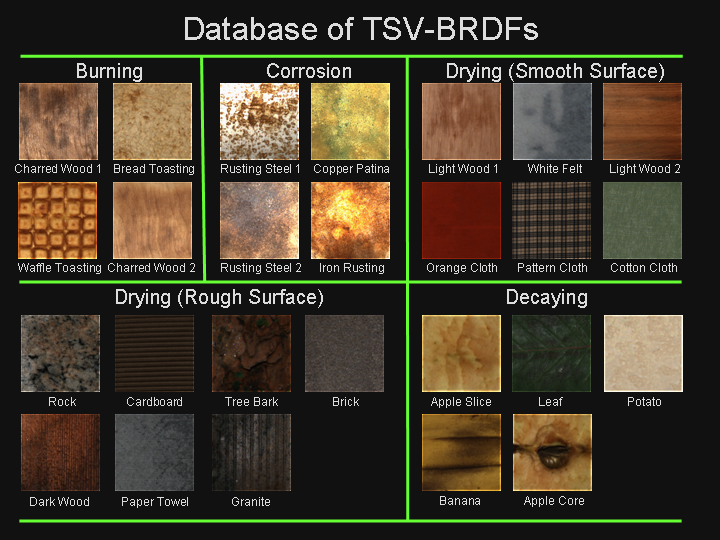
\includegraphics[width=0.75\textwidth]{figures/database}
\end{center}
\caption{The STAF database contains various phenomena \cite{Gu2006}.}
\label{Fig:Database}
\end{figure}

\section{Texture Synthesis}


\section{Conclusion}

\vspace{3.0cm}

\bibliographystyle{plain}
\bibliography{reference}


\end{document}

